\section{Analisi del dominio}

Il risultato dell'analisi del dominio dei giochi da tavolo è rappresentato in Figura \ref{fig:domain_analysis}.
%
L'analisi ha evidenziato la presenza costante di una divisione in \textbf{aspetti intensionali}, ovvero fissati indipendentemente da una specifica partita, ed \textbf{aspetti estensionali}, che catturano dettagli legati al gioco durante il suo svolgimento.

\begin{figure}
  \centering
  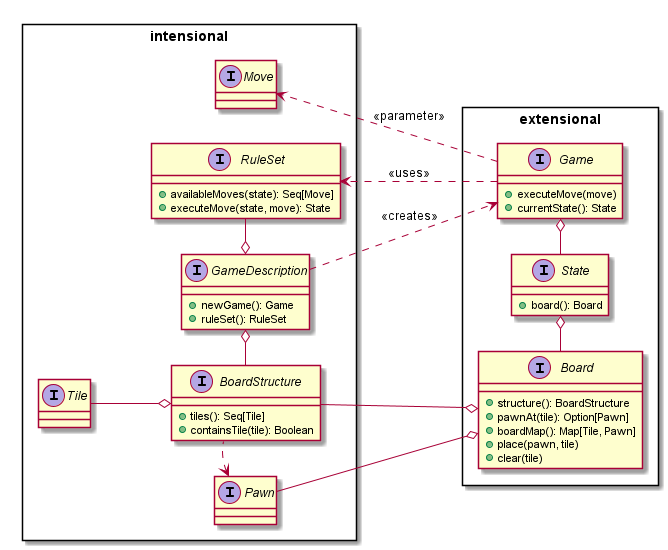
\includegraphics[width=\linewidth]{images/uml/domain_analysis.png}
  \caption{Diagramma delle classi rappresentante il risultato dell'analisi del modello del dominio}
  \label{fig:domain_analysis}
\end{figure}

\subsection{Aspetti intensionali}
I concetti intensionali sono visibili nella porzione di sinistra del diagramma in Figura \ref{fig:domain_analysis}.

Il nucleo di questo insieme di entità è costituito dalla \texttt{GameDescription}, che rappresenta la definizione principale di un gioco e viene utilizzata per crearne nuove istanze.
%
Ad ogni \texttt{GameDescription} è associato un \texttt{RuleSet}, che contiene la logica per la generazione e l'esecuzione delle mosse disponibili per un dato stato della partita, e una \texttt{BoardStructure} contenente la disposizione dei \texttt{Tile} che costituiscono il tabellone di gioco e il tipo di \texttt{Pawn} che possono ospitare.

Infine, fanno parte degli aspetti intensionali anche le \texttt{Move}, che racchiudono tutte le informazioni necessarie al \texttt{RuleSet} per l'esecuzione della mossa stessa.

\subsection{Aspetti estensionali}
A livello estensionale, le entità individuate sono collocate nella metà di destra del diagramma in Figura \ref{fig:domain_analysis}.

La radice di questo gruppo di entità è il \texttt{Game}, ovvero la rappresentazione di una istanza attiva di partita.
%
Ad esso è affidato il compito di mantenere consistente lo \texttt{State} della partita a fronte dell'esecuzione delle \texttt{Move} e utilizza quindi il \texttt{RuleSet} per garantire questa proprietà.

Uno \texttt{State} contiene tutte le informazioni necessarie a definire un istante legale del proseguimento della partita, comprendente di stato della \texttt{Board}, giocatori attivi, turno corrente, ecc.
%
Non tutti questi aspetti sono condivisi da tutti i giochi da tavolo, e sono perciò omessi nel diagramma ad eccezione della \texttt{Board}, che è sempre presente.

Infine, la \texttt{Board} è l'entità che definisce e manovra la disposizione dei \texttt{Pawn} sui \texttt{Tile} definiti dalla sua \texttt{BoardStructure}.
%
La \texttt{Board} deve anche imporre il vincolo di avere al più un \texttt{Pawn} su ogni \texttt{Tile}.

\subsection{Aspetti comuni dei giochi da tavolo}
%
Si analizzano ora gli aspetti trasversali a tutti i giochi da tavolo.
%
\paragraph{Turni e Giocatori}
%
I giochi da tavolo sono quasi sempre suddivisi in turni che scandiscono il flusso di una partita; un turno solitamente identifica una serie di azioni le quali possono essere svolte prima della sua terminazione.
%
Ogni gioco, inoltre, ha un numero fissato di giocatori che prendono parte ad una partita (un gioco con zero giocatori è da intendersi come un simulatore e non più un gioco).
%
Il sistema dei turni e quello dei giocatori sono quasi sempre fortemente legati tra loro e in molti casi i concetti di turno e di giocatore sono sovrapposti e interscambiabili.
%
\paragraph{Condizioni di terminazione}
%
Queste identificano l'insieme di condizioni necessarie e sufficienti affinchè una partita termini.
%
Le partite possono terminare solitamente in due modi:
\begin{itemize}
  \item vittoria di un giocatore: caso in cui un giocatore ha raggiunto i requisisti per essere dichiarato vincitore.
  \item pareggio: caso in cui nessun giocatore è dichiarato vincitore e la partita non può proseguire.
\end{itemize}